\documentclass[10pt]{article}
\usepackage[english]{babel}
\usepackage[utf8x]{inputenc}
\usepackage[T1]{fontenc}
\usepackage{scribe}
\usepackage{listings}

\lstset{style=mystyle}
\setlength\parindent{0pt}
\begin{document}
\MakeScribeTop{Market MicroStructure (MM)}{Optimal Execution of Portfolio Transactions}{Robert Almgren and Neil Chriss - December 2000}
%#############################################################
%#############################################################
%#############################################################
%#############################################################



\section{Introduction} 

\subsection{Portfolio Liquidation}

\textbf{Financial problem}

\begin{itemize} 
    \item We want to sell a large quantity of a stock (or of several stocks) in one day.
    \item How to choose the transaction times?
\end{itemize}

\subsection{Strategies (1)}

\textbf{Naive strategies}

\begin{itemize} 
    \item 2 extreme strategies:
    \begin{itemize} 
        \item Sell everything right now $\rightarrow$ huge transaction cost since we need to "eat" a lot in the order book. However this cost is known.
        \item Sell regularly in the day small amounts of assets $\rightarrow$ small transaction costs (volumes are much smaller) but the final profit is unknown because of the daily price fluctuations :
        Volatility risk.
    \end{itemize}
\end{itemize}

\subsection{Strategies (2)}

\textbf{Optimization}

\begin{itemize} 
    \item We need to optimize between transaction costs and volatility risk.
    \item To do so, we use the Almgren and Chriss framework which takes into account the market impact phenomenon and emphasizes the importance of having good statistical estimators of market parameters.
\end{itemize}

\section{Almgren and Chriss model}

\subsection{Trading strategy}

\textbf{Setup}

\begin{itemize} 
    \item We consider we are selling one asset. We have $X$ shares of this assets at $t_{0}=0$
    \item We want everything to be sold at $t=T$.
    \item We split $[0, T]$ into $N$ intervals of length $\tau=T / N$ and set $t_{k}=k \tau, k=0, \ldots, N$
    \item A trading strategy is a vector $\left(x_{0}, \ldots, x_{N}\right)$, with $x_{k}$ the number of shares we still have at time $t_{k}$.
    \item $x_{0}=X, x_{N}=0$ and $n_{k}=x_{k-1}-x_{k}$ is the number of assets sold between $t_{k-1}$ and $t_{k}$, decided at time $t_{k-1}$.
\end{itemize}

\subsection{Price decomposition}

\textbf{Price components}

\begin{itemize} 
    \item The price we have access to moves because of :
    \begin{itemize} 
        \item The drift $\rightarrow$ negligible at the intraday level.
        \item The volatility.
        \item The market impact.
    \end{itemize}
\end{itemize}

\subsection{Permanent market impact}

\textbf{Permanent impact component}

\begin{itemize} 
    \item Market participants see us selling large quantities.
    \item Thus they revise their prices down.
    \item Therefore, the "equilibrium price" of the asset is modified in permanent way.
    \item Let $S_{k}$ be the equilibrium price at time $t_{k}$ :
    $$
    S_{k}=S_{k-1}+\sigma \tau^{1 / 2} \xi_{k}-\tau g\left(n_{k} / \tau\right)
    $$
    \item with $\xi_{k}$ iid standard Gaussian and $n_{k} / \tau$ the average trading rate between $t_{k-1}$ and $t_{k}$.
\end{itemize}

\subsection{Temporary market impact}

\textbf{Temporary impact component}

\begin{itemize} 
    \item It is due to the transaction costs: we are liquidity taker since we "eat" the order book.
    \item If we sell a large amount of shares, our price per share is significantly worse than when selling only one share.
    \item We assume this effect is temporary and the liquidity comes back after each period.
    \item Let $\tilde{S}_{k}=\left(\sum n_{k, i} p_{i}\right) / n_{k}$, with $n_{k, i}$ the number of shares sold at price $p_{i}$ between $t_{k-1}$ and $t_{k} .$ We set
    $$
    \tilde{S}_{k}=S_{k-1}-h\left(n_{k} / \tau\right)
    $$
    \item The term $h\left(n_{k} / \tau\right)$ does not influence the next equilibrium price $S_{k}$.
\end{itemize}

\subsection{Profit and Loss}

\textbf{Cost of trading}

\begin{itemize} 
    \item The result of the sell of the asset is
    $$
    \begin{array}{c}
    \sum_{k=1}^{N} n_{k} \tilde{S}_{k} \\
    =X S_{0}+\sum_{k=1}^{N}\left(\sigma \tau^{1 / 2} \xi_{k}-\tau g\left(n_{k} / \tau\right)\right) x_{k}-\sum_{k=1}^{N} n_{k} h\left(n_{k} / \tau\right)
    \end{array}
    $$
    \item The trading cost $\mathcal{C}=X S_{0}-\sum_{k=1}^{N} n_{k} \tilde{S}_{k}$ is equal to
    Vol. cost $+$ Perm. Impact cost $+$ Temp. Impact cost.
\end{itemize}

\subsection{Mean-Variance analysis}

\textbf{Moments}

\begin{itemize} 
    \item Consider a static strategy (fully known in $\left.t_{0}\right)$, which is in fact optimal in this framework. We have
    $$
    \mathbb{E}[\mathcal{C}]=\sum_{k=1}^{N} \tau x_{k} g\left(n_{k} / \tau\right)+\sum_{k=1}^{N} n_{k} h\left(n_{k} / \tau\right), \quad \operatorname{Var}[\mathcal{C}]=\sigma^{2} \sum_{k=1}^{N} \tau x_{k}^{2}
    $$
    \item In order to build optimal trading trajectories, we will look for strategies minimizing
    $$
    \mathbb{E}[\mathcal{C}]+\lambda \operatorname{Var}[\mathcal{C}]
    $$
    with $\lambda$ a risk aversion parameter.
\end{itemize}

\section{Naive strategies}

\subsection{Assumptions (1)}

\textbf{Permanent impact}

\begin{itemize} 
    \item Linear permanent impact: $g(v)=\gamma v$.
    \item If we sell $n$ shares, the price per share decreases by $\gamma n .$ Thus
    $$
    S_{k}=S_{0}+\sigma \sum_{j=1}^{k} \tau^{1 / 2} \xi_{j}-\gamma\left(X-x_{k}\right)
    $$
    \item and in $\mathbb{E}[\mathcal{C}]$, the permanent impact component satisfies
    $$
    \sum_{k=1}^{N} \tau x_{k} g\left(n_{k} / \tau\right)=\gamma \sum_{k=1}^{N} x_{k}\left(x_{k-1}-x_{k}\right)=\frac{1}{2} \gamma X^{2}-\frac{1}{2} \gamma \sum_{k=1}^{N} n_{k}^{2}
    $$
\end{itemize}

\subsection{Assumptions (2)}

\textbf{Temporary impact}

\begin{itemize} 
    \item Affine temporary impact: $h\left(n_{k} / \tau\right)=\varepsilon+\eta\left(n_{k} / \tau\right)$.
    \item $\varepsilon$ represents a fixed cost : fees $+$ bid ask spread.
    \item Let $\tilde{\eta}=\eta-\frac{1}{2} \gamma \tau$, we get
    $$
    \mathbb{E}[\mathcal{C}]=\frac{1}{2} \gamma X^{2}+\varepsilon X+\frac{\tilde{\eta}}{\tau} \sum_{k=1}^{N} n_{k}^{2}
    $$
\end{itemize}

\subsection{Regular liquidation}

\textbf{Regular strategy}

\begin{itemize} 
    \item Take $n_{k}=X / N, x_{k}=(N-k) X / N, k=1, \ldots, N$.
    \item We easily get
    $$
    \begin{array}{l}
    \mathbb{E}[\mathcal{C}]=\frac{1}{2} \gamma X^{2}+\varepsilon X+\tilde{\eta} \frac{X^{2}}{T} \\
    \operatorname{Var}[\mathcal{C}]=\frac{\sigma^{2}}{3} X^{2} T\left(1-\frac{1}{N}\right)\left(1-\frac{1}{2 N}\right) .
    \end{array}
    $$
    \item We can show this strategy has the smallest expectation. However the variance can be very big if $T$ is large.
\end{itemize}

\subsection{Immediate selling}

\textbf{Selling everything at t0}

\begin{itemize} 
    \item Take $n_{1}=X, n_{2}=\ldots=n_{N}=0, x_{1}=\ldots=x_{N}=0$
    \item We get
    $$
    \begin{array}{l}
    \mathbb{E}[\mathcal{C}]=\varepsilon X+\frac{\eta X^{2}}{\tau} \\
    \operatorname{Var}[\mathcal{C}]=0
    \end{array}
    $$
    \item This strategy has the smallest variance. However, if $\tau$ is small, the expectation can be very large.
\end{itemize}

\section{Optimal strategies}

\subsection{Optimization (1)}

\textbf{Optimization program}

\begin{itemize} 
    \item - The trader wants to minimize
    $$
    U(\mathcal{C})=\mathbb{E}[\mathcal{C}]+\lambda \operatorname{Var}[\mathcal{C}] .
    $$
    \item $U(\mathcal{C})$ is equal to
    $$
    \frac{1}{2} \gamma X^{2}+\varepsilon X+\frac{\tilde{\eta}}{\tau} \sum_{k=1}^{N}\left(x_{k-1}-x_{k}\right)^{2}+\lambda \sigma^{2} \sum_{k=1}^{N} \tau x_{k}^{2}
    $$
\end{itemize}

\subsection{Optimization (2)}

\textbf{Derivation}

\begin{itemize} 
    \item For $j=1, \ldots, N-1$,
    $$
    \frac{\partial U}{\partial x_{j}}=2 \tau\left(\lambda \sigma^{2} x_{j}-\tilde{\eta} \frac{\left(x_{j-1}-2 x_{j}+x_{j+1}\right)}{\tau^{2}}\right)
    $$
    \item Therefore
    $$
    \frac{\partial U}{\partial x_{j}}=0 \Leftrightarrow \frac{\left(x_{j-1}-2 x_{j}+x_{j+1}\right)}{\tau^{2}}=\tilde{K} x_{j}
    $$
    with $\tilde{K}=\lambda \sigma^{2} / \tilde{\eta}$.    
\end{itemize}

\subsection{Optimization (3)}

\textbf{Solution}

\begin{itemize} 
    \item It is shown that the solution can be written $x_{0}=X$ and for $j=1, \ldots, N:$
    $$
    \begin{array}{l}
    x_{j}=\frac{\sinh \left(K\left(T-t_{j}\right)\right)}{\sinh (K T)} X \\
    n_{j}=\frac{2 \sinh (K \tau / 2)}{\sinh (K T)} \cosh (K(T-j \tau+\tau / 2))
    \end{array}
    $$
    where $K$ satisfies $\frac{2}{\tau^{2}}(\cosh (K \tau)-1)=\tilde{K}$
    \item If $\lambda=0$, then $\tilde{K}=K=0$ and so $n_{j}=\tau / T=X / N$. We retrieve the strategy with minimal expected cost.
\end{itemize}

\subsection{Remarks on this approach}

\textbf{Remarks}

\begin{itemize} 
    \item It is easy to show that the solution is time homogenous: if we compute the optimal strategy in $t_{k}$, we obtain the value between $t_{k}$ and $T$ of the optimal strategy computed in $t_{0}$.
    \item In this approach, we obtain an efficient frontier of trading.
    \item The optimal trajectories are very sensitive to the volatility parameter. It is therefore important to obtain accurate volatility estimates.
    \item The Almgren and Chriss framework can be extended in dimension $n$ (if we sell several assets). In that case, correlation parameters come into the picture.
\end{itemize}

\subsection{Results}

\textbf{Optimal Trajectory for a Single-Asset Portfolio}

\begin{center} 
    \begin{figure}[hbt!]
        \captionsetup{justification=centering,margin=0.5cm}
        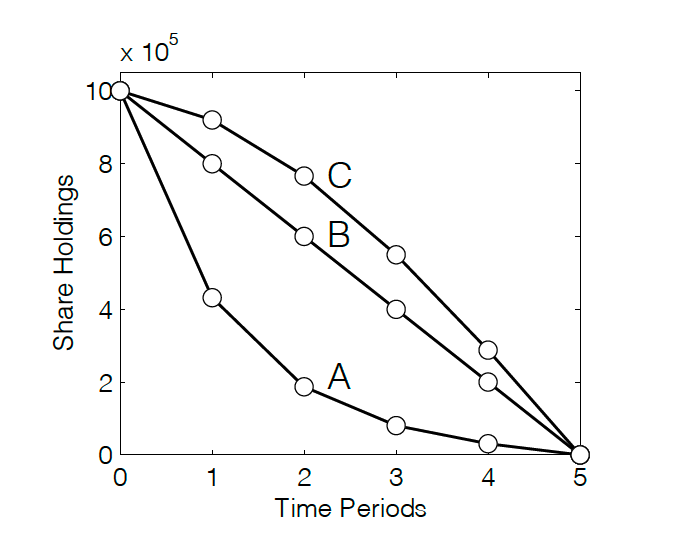
\includegraphics[width=13cm,height=4cm,keepaspectratio,]{op1.png}
        \centering
        \caption[caption]{Optimal trajectories. The trajectories corresponding to the points shown in Figure 1. (A) $\lambda=2 \times 10^{-6},\left(\right.$ B) $\lambda=0,\left(\right.$ C) $\lambda=-2 \times 10^{-7}$.
        \cite[p.18]{Almgren_optimalexecution}}
    \end{figure}
\end{center}

\textbf{Optimal Trajectories for the liquidation of a Two-Asset Portfolio}

\begin{center} 
    \begin{figure}[hbt!]
        \captionsetup{justification=centering,margin=0.5cm}
        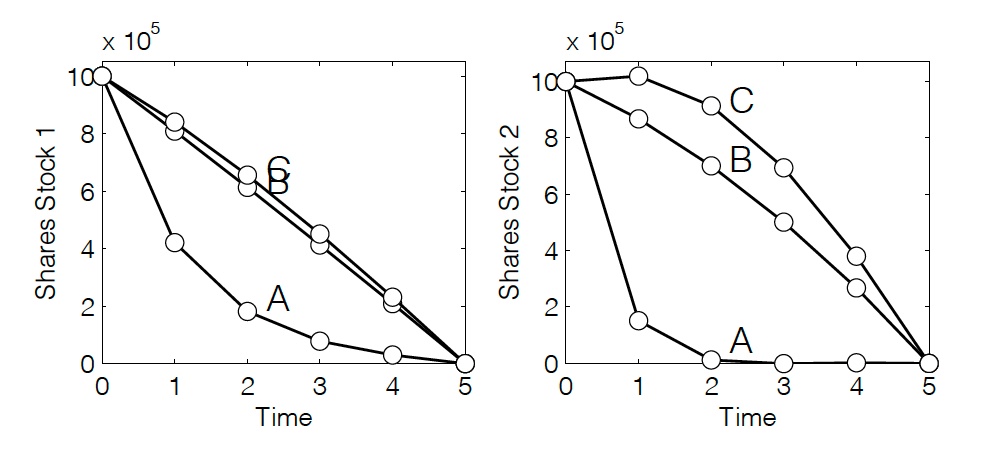
\includegraphics[width=13cm,height=4cm,keepaspectratio,]{op2.png}
        \centering
        \caption[caption]{Optimal trajectories for two securities. As in Figure 5 , for (A) $\lambda=2 \times 10^{-6},(\mathrm{~B})$ the naïve strategy with $\lambda=0,(\mathrm{C}) \lambda=-5 \times 10^{-8}$.
        \cite[p.41]{Almgren_optimalexecution}}
    \end{figure}
\end{center}

\bibliographystyle{abbrv}           
\bibliography{./myref.bib}
\end{document}